
\graphicspath{ {3chapterTheory/image/} }
\chapter{Theoretical Background}
\section{Mathematical morphology}
%------------------------------------------------------------
%--------
%------------------------------------------------------------
Morphology come from Greek and means the "study of shape". Mathematical Morphology (MM) deals with describing shapes based on the set theory, integral geometry and lattice algebra. It is not just a theory but is now part of classical powerful image processing techniques. In the field of document image processing and analysis, in which the shape of objects contains prominent features, some morphological operators are regularly used. Mathematical morphology contains non-linear operator that can transform the shape of objects, thus allowing to extract them. Morphological operators can be classified as follow:
\begin{enumerate}
\item \textbf{Operators of binary images based on structuring element}. These operators describe the interaction of an image with a structuring element S. A binary image $1_F$: $ D \rightarrow \mathbb{B} $ is the indicator function of a set of point F which is a subset of and Euclidean space $ \mathbb{R}^d $ or the integer grid $\mathbb{Z}^d$ of dimension d. A structuring element is a set \textit{S}, usually centered in a limited definition domain. It acts like a filter for any transform applying to \textit{F}. The size of S, usually small relative to the images, affects the strength of the transform and its sharp defines how the transform modify the shape of components in image. Many morphological operators has been defined, some of them are dual by set complementation. Two famous morphology operators, erosion and dilation, belong to this class. Erosion is defined as $ \epsilon_S (F) = \lbrace p  \vert  \forall s \in S, p + s \in F\rbrace $  and dilation is defined as $ \delta_S (F) = \lbrace p+s  \vert  \forall p \in F, s \in S\rbrace $ Their effects can be seen in \ref{fig:erosionbin} and \ref{fig:dilationbin}. They are dual operators with respect to complementation $ \epsilon_S (F) = \mathcal{C} {\delta_{S}\mathcal{C}F} $ . This duality property illustrates the fact that erosion and dilation do not process the objects and their background symmetrically: the erosion shrinks the objects but expands their background (and vice versa for the dilation).
\par Other interesting morphological filters can be formed using the differences of two or more operators, for example the morphological gradient and morphological Laplacian. As the erosion shrinks objects and the dilation grows them, examining the difference between original image and its erosion and dilation can gave us information of the edge of objects. The morphological gradient defined by $\triangledown_S (F) = \delta_S (F) - \epsilon_S (F) $. This thick gradient appears on two sides of the acture edges and can be decomposed into two half gradient $\triangledown_S (F) = \triangledown_S ^- (F) + \triangledown_S ^+ (F)$ with $ \triangledown_S ^- (F) = F - \epsilon_S (F)$ is the inner gradient adheres to insides of objects and $ \triangledown_S ^+ (F) =\delta_S (F) - F$ is the outer gradient, adheres to the outside of objects. The morphological equivalent of the Laplacian is defined by $\vartriangle_S (F) =\triangledown_S ^+ (F) - \triangledown_S ^- (F)=\delta_S (F)+\epsilon_S (F) - 2F$. There effects are shown in \ref{fig:gradientbin}, \ref{fig:gradientInbin}, \ref{fig:gradientOutbin} and \ref{fig:laplacianbin}

\begin{figure}
	\begin{subfigure}{0.2\textwidth}
	 	
\includegraphics{bin/input.png} \caption{Input F}\label{fig:inputbin} \end{subfigure}
	\begin{subfigure}{0.2\textwidth}
	 	
\includegraphics{bin/erosion.png} \caption{$ \epsilon_S (F)$}\label{fig:erosionbin} \end{subfigure}
	\begin{subfigure}{0.2\textwidth}
		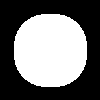
\includegraphics{bin/dilation.png} \caption{$ \delta_S (F)$}\label{fig:dilationbin} \end{subfigure}
	\centering
		
	\begin{subfigure}{0.2\textwidth}
		
\includegraphics{bin/gradient.png} 
		\caption{$ \triangledown_S (F)$}\label{fig:gradientbin} \end{subfigure}
	\begin{subfigure}{0.2\textwidth}
		
\includegraphics{bin/gradientIn.png} 
		\caption{$ \triangledown_S ^- (F)$}\label{fig:gradientInbin} \end{subfigure}		
	\begin{subfigure}{0.2\textwidth}	
		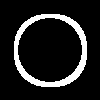
\includegraphics{bin/gradientOut.png} 
		\caption{$ \triangledown_S ^+ (F)$}\label{fig:gradientOutbin} \end{subfigure}
	\begin{subfigure}{0.2\textwidth}	
		
\includegraphics{bin/laplacian.png} 
		\caption{$\vartriangle_S (F)$}\label{fig:laplacianbin} \end{subfigure}					
	\centering
	\caption[Example of \textit{morphological operations}] {Binary Morphological Operations. The morphological Laplacian is colorized by Green (positive), red (negative) and black (zero) }
	\label{fig:binOperations}
\end{figure}


\item \textbf{Elementary operators of binary images  on sets}. By replacing the structuring element B by the notion of neighborhood $\mathcal{N}$, morphological operators obtained will have elementary behavior (the slightest transform effect possible). For example, $ \delta_\mathcal{N} (F) = \lbrace p' \in \mathcal{N}(p) \cup p  \vert  p \in F \rbrace $ is the elementary dilation.

\item \textbf{Extension from sets to functions} of the first two categories. Applying threshold decomposition principle, morphological operators can be extended to function i.e gray level images. $ f: \mathcal{D} \rightarrow \mathbb{N}$. With a gray level t given, the subset of $ \mathcal{D} $ obtained by shareholding f by t is denoted by $[f \geq t] = \lbrace p \in \mathcal{D} \vert f(p) \geq t \rbrace $. Any morphological set operator $\phi^{set}$ can be extended to define a morphological operator on gray level function $\phi$ using $ \phi(f)(p) = max \lbrace t \vert p \in \phi^{set}([f \geq t]) \rbrace $. There effect can be seen in \ref{fig:grayLevelOperations}.

\begin{figure}
	\begin{subfigure}{0.2\textwidth}
	 	
\includegraphics{grayLevel/input.png} \caption{Input F}\label{fig:inputgrayLevel} \end{subfigure}
	\begin{subfigure}{0.2\textwidth}
	 	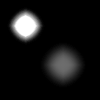
\includegraphics{grayLevel/erosion.png} \caption{$ \epsilon_S (F)$}\label{fig:erosiongrayLevel} \end{subfigure}
	\begin{subfigure}{0.2\textwidth}
		
\includegraphics{grayLevel/dilation.png} \caption{$ \delta_S (F)$}\label{fig:dilationgrayLevel} \end{subfigure}
	\centering
		
	\begin{subfigure}{0.2\textwidth}
		
\includegraphics{grayLevel/gradient.png} 
		\caption{$ \triangledown_S (F)$}\label{fig:gradientgrayLevel} \end{subfigure}
	\begin{subfigure}{0.2\textwidth}
		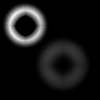
\includegraphics{grayLevel/gradientIn.png} 
		\caption{$ \triangledown_S ^- (F)$}\label{fig:gradientIngrayLevel} \end{subfigure}		
	\begin{subfigure}{0.2\textwidth}	
		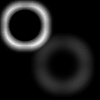
\includegraphics{grayLevel/gradientOut.png} 
		\caption{$ \triangledown_S ^+ (F)$}\label{fig:gradientOutgrayLevel} \end{subfigure}
	\begin{subfigure}{0.2\textwidth}	
		
\includegraphics{grayLevel/laplacian.png} 
		\caption{$\vartriangle_S (F)$}\label{fig:laplaciangrayLevel} \end{subfigure}					
	\centering
	\caption[Example of \textit{morphological operations}] {Morphological Operations on set, using a square 10x10 pixels as the structuring element. (The laplacian is colorized by Green (positive), red (negative) and black (zero)) }
	\label{fig:grayLevelOperations}
\end{figure}


\item \textbf{Connected operators}. Connected operators \cite{Salembier95flatzones} are operator that work by merging elementary region called flat zones. It verify 
$ \forall p, \forall p' \in \mathcal{N}(p), f(p')=f(p) \Longrightarrow  \phi(f)(p')=\phi(f)(p)$. As a consequence, connecting operators cannot create new contours, nor modify their position. Therefore, they have a very good contour preservation properties. There are two commonly used classes of connected operators: filters by reconstruction and algebraic openings and closings \cite{Vincent.1993.tip}. Although they are well-know in the binary case, where only objects "marked" by another image are extracted, they can be defined for gray level images by shareholding the input image at different level t. \fxnote{example} 
\end{enumerate}
\par Mathematical Morphology is a powerful tool for image processing. It found application in numerous field: geoscience and remote sensing, materials science, biological and medical imaging, industrial applications, identification and security control, document processing and image coding \cite{Soille:2003:MIA:773286}. 


\section{Digital Topology and Self-Duality}
\par 
In the case of text detection in gray scale image, a well known problem encountered is to treat bright texts over dark background and dark texts over bright background. Common workaround which processes both the original and it complement will increase computation cost. Consequently, we interest in the class of self-dual operator.
\par
A self-dual operator processes the image contents regardless its contrast \cite{geraud.15.ismm}. In general, operators which are not self-dual do not treat bright objects over dark background and dark objects over bright background similarly which is often an undesirable feature. It is most important when no assumption about the contrast between object and background can be made. As any part of the images could be the subject, we want an operation which behavior the same way regardless the contrast between the subject and its background to obtain a unique representation.  
\begin{figure}

	\begin{subfigure}{0.3\textwidth}
	 	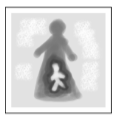
\includegraphics{im1.png} \caption{}\label{fig:gray} \end{subfigure}
	\begin{subfigure}{0.3\textwidth}
		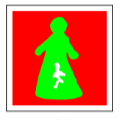
\includegraphics{im2.png} \caption{}\label{fig:mother} \end{subfigure}
	\begin{subfigure}{0.3\textwidth}
		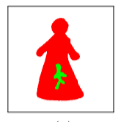
\includegraphics{im3.png} \caption{}\label{fig:baby} \end{subfigure}
	\centering
	\caption[Example of \textit{subjects}] {From the original gray level image \ref{fig:gray}, the subject can be either the mother \ref{fig:mother} (dark over bright) or the baby \ref{fig:baby} (bright over dark) }
	\label{fig:motheAndBaby}
\end{figure}

\par
As we can seen in \ref{fig:motheAndBaby}, where green and red respectively represent the background and foreground. From the grayscale image \ref{fig:gray} If we focus in the mother, then the outer zone will be the background as in \ref{fig:mother}. Furthermore, we can chose the baby as the subject and therefore, the woman will become the background \ref{fig:baby}.	
\par
For a image defined in the regular cubical grid, the digital topology must be describe by a "Jordan pair" of connectivity $(c_\alpha,c_\beta)$ \cite{Kong:1989:DTI:71397.71400}. One connectivity is used for the object and the other one for the background. 
\fxnote{connectivity image}
\par 
For example, if the image \ref{fig:topo} is describe by the pair $(c_4,c_8)$ (the 4-connectivity for bright pixel and 8-connectivity for dark pixel) we will obtain 1 object. On the same image, using $(c_8,c_4)$ will gave us 2 separate object. This arbitrary choice affect the topology and self-dual operation must use different connectivity for the complementary to work in the same way. It is demonstrated in \ref{fig:topoa} \ref{fig:topoc}: the complement image must use the $(c_8,c_4)$ connectivity to gave the same presentation of the original image which use $(c_4,c_8)$. This lead to the study of an image class which enjoys very useful topological and geometric properties: the well-composed images

\section{Well-composed Images}
\fxnote{about well-composed images}
\par
As defined in \cite{Latecki95}, a 2D set S is weakly well-composed if any 8-component of S is a 4 component. S is well-composed if both S and its complement $\bar{C}$ are weakly well-composed. It can easily be defined using the notion of "critical configurations" which are 
\includegraphics{confi1.jpg} and 
\includegraphics{confi2.jpg} : S is weakly well-composed if these configuration do not appear.
\par
The notion of well-composednessed has also been extended to gray-level images. A gray-level image $\mu$ is well-composed if any set $[\mu \geq \lambda ]$ is well-composed. The extended version of "critical configuration" is that every block 
\begin{tabular}{|c|c|}
\hline 
a & d \\ 
\hline 
c & b \\ 
\hline 
\end{tabular} 
must verify interval(a,b) $\cap$ interval(c,d) $\neq \varnothing$ , where interval(a,b) = [min(a,b),max(a,b)].
\par
An image is not a priori well-composed. There are 2 approach to get a well-composed image from the original image \cite{geraud.15.ismm} by changing it pixel value (with possibility of alter the image's topology) or by a well-composed interpolation.
\fxnote{attribute, important why we have to interpolate}


\section{Connected filter}
Motivated by families of filters by reconstruction, the notion of filter by reconstruction is introduced in \cite{Salembier95flatzones} \cite{Serra1993}. It work by simplifier the topographic map of images. The most important feature of this type of operator is preservation of contours \cite{Salembier2009}: they does not create new contours nor shift them.
\subsection{Morphological Tree-Based Image Representation}
One strategy to define connected operators replies on a hierarchical region-based representation of the input image, in another word, a tree. The filtering step is done by pruning that tree and the output image is compute by reconstructing the pruned tree.  Tree of shapes is a contrast-invariant image representation which is defined in \cite{Monasse.2000}.
\paragraph{} \textbf{A Couple of Dual Trees}: given an image $\mu $ in nD: $\mathbb{Z}^{n} \rightarrow \mathbb{Z} $, the lower cuts of $\mu$ are defined by 
	$[\mu < \lambda] =\lbrace x \in X \vert \mu (x) < \lambda \rbrace $. The set of all connected components of all these cuts is $ \mathcal{T}_< (\mu) =\lbrace \Gamma \in \mathcal{C}\mathcal{C}([\mu < \lambda]) \rbrace $ (with $\mathbb{C}\mathbb{C}$ denote the operator that takes a set and gives its set of connected component. As these sets verify $\forall \Gamma$ and $\Gamma ' \neq \lambda$, $\Gamma \subset \Gamma ' $ or $\Gamma \cap \Gamma '= \emptyset$, they can be arranged into a tree, called the \textit{min-tree} (because it if form using lower cuts, and the leaves will be minimum of image). We can also consider the upper cuts $[\mu \geq \lambda] =\lbrace x \in X \vert \mu (x) \geq \lambda \rbrace $, the element of $ \mathcal{T}_\geq (\mu) =\lbrace \Gamma \in \mathcal{C}\mathcal{C}([\mu \geq \lambda]) \rbrace $ will be arranged in to the \textit{max-tree}. The \textit{max-tree} and \textit{min-tree} are dual by complementation, the max-tree of $\mu$ is the min-tree of $ \mu$, therefore operations define on them are dual.
	
\paragraph{} \textbf{A Self-Dual Tree}:We use two set $ \mathcal{T}_< (\mu)$ and $ \mathcal{T}_\geq (\mu)$ with their holes filled to define two other sets $ \mathcal{S}_< (\mu)$ and $ \mathcal{S}_< (\mu)$. We denote \textit{Sat} as the cavity-fill-in operator, these new sets are defined as: $ \mathcal{S}_< (\mu) = \lbrace Sat(\Gamma);\Gamma \in \mathcal{T}_<(\mu)\rbrace$ and $ \mathcal{S}_\geq (\mu) = \lbrace Sat(\Gamma);\Gamma \in \mathcal{T}_\geq (\mu)\rbrace$. The tree of shape is defined as: $\mathfrak{S}(\mu) = \mathcal{S}_< (\mu) \bigcup \mathcal{S}_\geq (\mu) $. We have also $\Gamma \subset \Gamma ' $ or $\Gamma \cap \Gamma '= \emptyset$ with $\Gamma , \Gamma ' \in \mathcal{S}$. There is a quasi-linear algorithm to compute the tree of shape, which works also in the case of nD presented in \cite{geraud.13.ismm}. This tree is \textit{self-dual} because many self dual operation can be defined in this tree \textit{<reading article>}.

The min and max tree are easily compute with a few line of code \cite{berger.07.icip} and the tree of shape can be obtain thanks to \cite{geraud.13.ismm}. The tree encoding is very compact in term of memory: the parenthood relationship between pixels is an image having the same size of the input. 

	
\paragraph{To be continue... (consider add the attribute and definition of Sat)}
